%
% c02-separation.tex
%
% (c) 2008 Prof Dr Andreas Mueller
% $Id: c02-separation.tex,v 1.3 2008/09/13 23:01:45 afm Exp $
%
\lhead{Separation der Variablen}
\rhead{}
\chapter{Separation der Variablen\label{chapter-separation}}
\index{Stroboskop}
\index{Eigenschwingung}
\index{stehende Welle}
\begin{figure}
\begin{center}
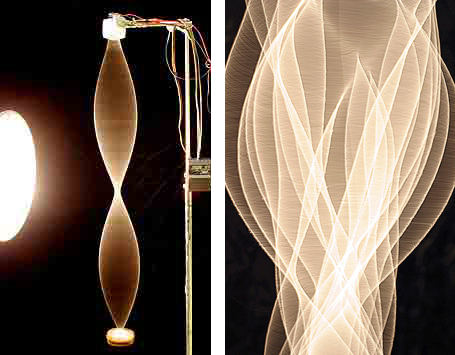
\includegraphics[width=0.8\hsize]{../common/graphics/stringvibrlarge-10-06-06.jpg}
\end{center}
\caption{Schwingende Saite (Bild von A.~Davidhazy, http://people.rit.edu/andpph/)
\label{separation:schwingendesaite}}
\end{figure}
Beleuchtet man eine schwingende Saite mit einem Stroboskop mit der
Frequenz der Eigenschwingung, scheint die Saite stillzustehen. 
In periodischen Zeit\-ab\-stän\-den sieht die Lösung der Wellengleichung
also gleich aus.
Misst man andererseits die Auslenkung der Saite
an einer Stelle in Abhängigkeit von der Zeit, beobachtet man
eine harmonische Schwingung, die sich mit Hilfe von $\sin$- und
$\cos$-Funktionen beschreiben lässt. Man kann also vermuten,
dass die Lösung der Wellengleichung der schwingenden Saite
ein Produkt
\[
u(x,t)=X(x)\cdot\sin\omega t\quad\text{oder}\quad X(x)\cdot\cos\omega t.
\]
ist. Ziel dieses Kapitels ist, diese Idee zu einem Lösungsverfahren
weiterzuentwickeln und auf einige Differentialgleichungen anzuwenden.

\section{Separation der Variablen für gewöhnliche Differentialgleichungen}
Die Differentialgleichung 
\begin{equation}
y'-xy=0
\label{separation:ode}
\end{equation}
kann mit Separation der Variablen gelöst werden:
\begin{align*}
\frac{dy}{dx}&=xy\\
\frac1y\,dy&=x\,dx\\
\int\frac1y\,dy&=\int x\,dx\\
\log|y|&=\frac12x^2+C\\
y&=y_0e^{\frac12x^2}
\end{align*}
Das Verfahren beruht auf dem Prinzip, auf jeder Seite der Gleichung
nur eine Variable zu haben.
Dabei zerlegt man sogar die Ableitung $dy/dx$, was man ja eigentlich
gar nicht darf.
Die Separation führt die Lösung der Differentialgleichung auf die
Berechnung zweier Integrale zurück, also eigentlich auf die
Lösung einer besonders einfachen Differentialgleichung der Form $y'=f(x)$
mit Lösung $y(x)=\int f(x)\,dx$.
Diese Form der Lösung sagt uns auch genau, was wir an Anfangsbedingungen
brauchen.
Ist $y_0$ der Wert der Lösung an der Stelle $x_0$, dann liefert
das Integral die Lösungsfunktion
\[
y(x)=\int_{x_0}^xf(\xi)\,d\xi + y_0.
\]

So einfach wird es für partielle Differentialgleichungen nicht sein.
Insbesondere für die an sich schon etwas ``anrüchige'' Operationen,
den Differentialquotienten $dy/dx$ auseinanderzureissen gibt es keinerlei
Entsprechung bei partiellen Ableitungen.
Unter geeigneten Voraussetzungen an das Gebiet und die Differentialgleichung
ist es aber immer noch denkbar, dass man die Variablen trennen kann,
also 
\[
\text{Funktionen/Ableitungen nur mit $x$} = \text{Funktionen/Ableitungen nur mit $y$}
\]
Da die linke Seite nur von $x$ abhängt, die rechte aber nur von $y$, müssen
beide Seiten konstant sein, die partielle Differentialgleichung zerfällt
in eine linke {\em gewöhnliche} Differentialgleichung für eine Funktion von
$x$ und eine rechte {\em gewöhnliche} Differentialgleichung für $y$.

Da wir über gewöhnliche Differntialgleichungen Bescheid wissen, sollte
es uns so möglich sein, eine partielle Differentialgleichung zu lösen
und herzuleiten, welche Art von Randwerten vorgegeben werden müssen, damit
die Differentialgleichung eindeutig lösbar ist.

\section{Idee des Verfahrens}
Oft hat man aus dem Anwendungsgebiet, aus dem eine partielle
Differentialgleichung stammt, Hinweise darauf, wie die Lösungsfunktion
von {\em einer} der unabhängigen Variablen abhängt.
Dann kann man Versuchen, die Lösung als Produkt oder Summe von
solchen ``vermuteten'' Funktionen darzustellen.

\index{Ansatz}
\index{Separationsansatz}
Aber selbst wenn man nichts über die Lösung weiss, kann man 
versuchen, die Lösung als Summe oder Produkt von Funktionen darzustellen,
die nur von jeweils einer Variablen abhängen. Als Beispiel versuchen
wir die lineare Differentialgleichung 
\begin{equation}
\frac1x
\frac{\partial u}{\partial x}
+
\frac1y
\frac{\partial u}{\partial y}
=\frac1{y^2}
,
\qquad x>1, y>1
\label{separation:beispiel1}
\end{equation}
zu lösen, wobei wir die Randbedingungen für den Moment ignorieren.
Wir versuchen, die Lösung als Summe von zwei Funktionen darzustellen,
welche nur von $x$ bzw.~$y$ abhängen, also
\begin{equation}
u(x,y)=X(x)+Y(y)
\quad\Rightarrow\quad
\begin{cases}
\quad{\displaystyle \frac{\partial u}{\partial x}}&=X'(x)\\
\\
\quad{\displaystyle \frac{\partial u}{\partial y}}&=Y'(y)\\
\end{cases}
\label{separation:beispiel1:ansatz}
\end{equation}
Setzt man dies in die Differentialgleichung (\ref{separation:beispiel1})
ein, erhalten wir die Gleichung
\[
\frac{X'(x)}{x}+\frac{Y'(y)}{y}=\frac1{y^2}
\]
oder
\begin{equation}
\frac{X'(x)}{x}
=\frac1{y^2}
-\frac{Y'(y)}{y}.
\label{separation:beispiel1:separiert}
\end{equation}
Die Form (\ref{separation:beispiel1:separiert}) hat eine besondere
Eigenschaft: die Variable $x$ kommt nur auf der linken Seite vor,
die Variable $y$ nur auf der rechten. Setzt man für $y$ irgend
einen Wert ein, verändert sich die rechte Seite nicht mehr,
die linke Seite muss also für alle $x$ den gleichen Wert geben.
Lässt man jetzt wieder das $y$ varieren, muss sich auch auf der rechten
Seite immer der gleiche Wert ergeben. Wir nennen den gemeinsamen Wert
$k$, und bekommen zwei gewöhnliche Differentialgleichungen
für $X(x)$ und $Y(y)$:
\begin{align}
\frac{X'(x)}{x}&=k
&
k&=\frac1{y^2}-\frac{Y'(y)}{y}
\label{separation:beispiel1:separiertedgl}
\end{align}
Die linke Differentialgleichung ist einfach zu lösen:
\begin{align*}
X'(x)&=kx\quad\Rightarrow\quad X(x)=
\frac12kx^2+C_x.
\end{align*}
Die rechte Differentialgleichung ist nur leicht komplizierter:
\begin{align*}
Y'(y)=\frac1y-ky
\quad\Rightarrow\quad
Y(y)=\int\frac1y-ky\,dy=
\log y-\frac12ky^2+C_y.
\end{align*}
Diese beiden Lösungen können wir jetzt wieder zu einer Lösung der
ursprünglichen Differentialgleichung zusammensetzen:
\begin{equation}
u(x,y)=
\frac12kx^2+
\log y-\frac12ky^2+C.
\label{separation:beispiel1:loesung}
\end{equation}
Wir haben damit eine unendliche Familie von Lösungen der
Differentialgleichung gefunden, für jedes Paar $(k,C)$ von
Parametern liefert die Formel (\ref{separation:beispiel1:loesung})
eine Lösung.
Dazu müssen wir in irgend einer Weise die Randbedingungen verwenden.
Damit haben wir eine Skizze für das Lösungsverfahren mit Separation:
\begin{enumerate}
\item Finde einen Lösungsansatz aus Funktionen, die nur von einer
Variablen abhängen.
\item Setze in die Differentialgleichung ein und separiere die Terme
so, dass zwei Variablen jeweils nur auf einer Seite vorkommen. Dann
hängen beide Seiten nicht mehr von dieser Variablen ab, jede Seite
ist eine Differentialgleichung mit weniger Variablen.
\item Löse die Teildifferentialgleichungen, und setze daraus 
Lösungen zusammen. 
\item Verwende die Randbedingungen, um eine Lösung zu finden.
\end{enumerate}
Wie man unschwer erkennen kann, ist weniger die Lösung der
einzelnen Teildifferentialgleichungen das Problem, sondern der letzte
Schritt. In den folgenden Abschnitten zeigen wir an Beispielen, wie
dies möglich ist.

\section{Separation für lineare partielle Differentialgleichungen}
Die Grundidee des Separationsverfahrens liefert eine Familie von Funktionen,
von ein paar Integrationskonstanten abhängen. Vorgegeben sind auf dem
Rand aber beliebige Funktionen, es ist im Allgemeinen nicht möglich,
durch richtige Wahl von wenigen Parametern beliebige Funktionen zu erhalten.
Des Separationsverfahren in der bisherigen Form kann also ein
beliebiges Randwertproblem noch nicht lösen.

Nehmen wir an, es müsse die Differentialgleichung $Lu=f$ auf dem
Gebiet $\Omega$ mit Randwerte $g(x)$ für $x\in\partial \Omega$
gelöst werden.
Wir haben nur dann eine Chance, aus den bisherigen Resultaten eine 
vollständige Lösung des Problems zu erhalten, wenn wir in der
Lage sind, solche Teillösungen zu einer vollständigen Lösung
zu kombinieren. Dazu sind aber im allgemeinen zusätzliche
Bedingungen an die Differentialgleichung nötig. Linearität der
Differentialgleichung ist, was wir hier verwenden wollen:

\begin{satz}Sind $u_1$ und $u_2$ Lösungen einer homogenen linearen partiellen
Differentialgleichung, dann sind auch $u_1+u_2$ und $\lambda u_1$ für
$\lambda\in\mathbb R$ Lösungen
\end{satz}

\begin{proof}[Beweis]
Die Differentialgleichung
\[
F(x_1,\dots,x_2,u,\frac{\partial u}{\partial x_1},\dots)=0
\]
ist linear in $u$ und den Ableitungen, man darf also Summen und Vielfache
in $u$ und den Ableitungen aus der Funktion herausziehen:
\begin{align*}
F(x_1,\dots,x_2,u_1+u_2,\frac{\partial u_1}{\partial x_1}+\frac{\partial u_2}{\partial x_1},\dots)
&=
F(x_1,\dots,x_2,u_1,\frac{\partial u_1}{\partial x_1},\dots)
\\
&+
F(x_1,\dots,x_2,u_2,\frac{\partial u_2}{\partial x_1},\dots)=0
\\
F(x_1,\dots,x_2,\lambda u_1,\frac{\partial \lambda u_1}{\partial x_1},\dots)
&=
\lambda
F(x_1,\dots,x_2,u_1,\frac{\partial u_1}{\partial x_1},\dots)
=0
\end{align*}
Die Linearkombinationen von $u_1$ und $u_2$ sind also auch Lösungen.
\end{proof}

Um die Differentialgleichung zu lösen, kann man also versuchen, mit
dem bisherigen Separationsverfahren möglichst viele Lösungen zu
$u_1$, $u_2$, $u_3,\dots$ zu finden, und diese dann zu einer Gesamtlösung
zu kombinieren
\[
u(x)=\sum_{i=1}^\infty a_ku_k
\]
mit geeigneten Koeffizienten $a_k$, die so zu wählen sind, dass die
Randbedingungen erfüllt sind.

Inhomogene lineare partielle Differentialgleichungen kann man mit diesem
Verfahren ebenfalls lösen. Dazu findet man zunächst eine partikuläre
Lösung $u_p$, welche die inhomogenen Differentialgleichung löst, ohne
allerdings korrekte Randwerte zu liefern.
Das ursprüngliche Separationsverfahren kann hierbei hilfreich sein.
Dann verwendet man das skizzierte Verfahren für homogene lineare
partielle Differentialgleichungen für modifizierte Randwerte $g-u_p$ auf
$\partial\Omega$ um eine Lösung der homogenen Gleichung $u_h$ zu finden.
Die Summe $u=u_p+u_h$ ist dann eine Lösung der inhomogenen Gleichung
mit Randwerten $u_p + (g-u_p)=g$, also ein Lösung des ursprünglichen
Problems.

Die Bestimmung der Koeffizienten $a_k$ für die gefundene Familie
von Teillösungen führt oft auf die Fourier-Theorie, oder allgemeiner
auf orthogonale Funktionenfamilien. Solche Teillösungen haben oft eine
unmittelbare physikalische Bedeutung, zum Beispiel treten sie auf als
Schiwngungsmoden (in der Mechanik oder Elektrotechnik) oder als
Elektronenzustände in der Quantenmechanik.

\section{Schwingende rechteckige Membran}
\rhead{Rechteckige Membran}
\index{Membran!rechteckig}
Wir betrachten die Schwingung einer rechteckigen Membran, die am Rande
des Gebietes
\[
R=\{(x,y)\,|\,0\le x\le a,0\le y\le b\} =(0,a)\times(0,b)
\]
eingespannt ist. Zur Zeit $t=0$ sei die Form der Membran durch die
Funktion $f(x,y)$ gegeben.
Für beliebige Zeit $t\ge 0$ wird sie beschrieben durch eine Funktion $u(x,y,t)$,
welche der Differentialgleichung
\[
\frac1{c^2}\frac{\partial^2u}{\partial t^2}=\frac{\partial^2u}{\partial x^2}+\frac{\partial^2u}{\partial y^2}
\]
genügt mit den Anfangsbedingungen
\begin{align*}
u(x,y,0)&=f(x,y)\quad\forall 0\le x\le a,0\le y\le b,
\\
\frac{\partial}{\partial t}u(x,y,0)&=g(x,y)\quad\forall 0\le x\le a,0\le y\le b
\end{align*}
und den Randbedingungen
\begin{align*}
u(0,y,t)&=0&u(a,y,t)&=0&\forall t\ge 0,0\le y\le b,\\
u(x,0,t)&=0&u(x,b,t)&=0&\forall t\ge 0,0\le x\le a.
\end{align*}

\subsection{Separation der Zeit}
\index{Separation}
Nach der in der Einleitung motivierten Idee suchen wir Lösungen also
Produkt einer Funktion $T(t)$, die nur von der Zeit abhängt, und einer Funktion
$\varphi(x,y)$, welche nur vom Ort abhängt, also
\[
u(x,y,t)=T(t)\cdot\varphi(x,y).
\]
Leider kann ein einzelnes solches Produkt nicht alle Anfangsbedingungen
erfüllen. Wäre dies nämlich möglich, müsste $\varphi(x,y)\sim f(x,y)$
sein und alle Teile der Membran würden im Gleichtakt hin und her schwingen.
Simulationen oder physikalische Experimente zeigen aber, dass es
Anfangsbedingungen gibt, bei denen die Teile der Membran gegenläufig
schwingen.

Anderseits, muss die Lösung auf jeden Fall die Randbedingung erfüllen,
es muss also gelten
\begin{align*}
\varphi(0,y)&=0&\varphi(a,y)&=0&0\le y\le b\\
\varphi(x,0)&=0&\varphi(x,b)&=0&0\le x\le a
\end{align*}
Setzen wir diesen Ansatz für $u$ in der Wellengleichung ein,
erhalten wir
\[
\frac1{c^2}T''(t)\varphi(x,y)=T(t)\left(
\frac{\partial^2\varphi}{\partial x^2}
+
\frac{\partial^2\varphi}{\partial y^2}
\right)
\]
Wir suchen eine Funktion $u$, die nicht identisch verschwindet,
es gibt also einige Zeitpunkte $t$ und Orte $(x,y)$, an denen $T(t)$
und $\varphi(x,y)$ nicht verschwinden. An diesen Stellen kann man die
Gleichung umformen in
\begin{equation}
\frac1{c^2}\frac{T''(t)}{T(t)}
= \frac1{\varphi(x,y)}\left( \frac{\partial^2\varphi}{\partial x^2}
+ \frac{\partial^2\varphi}{\partial y^2} \right)
\label{separiertMembran}
\end{equation}
Die rechte Seite hängt nur
vom Ort ab, darf sich also nicht ändern, wenn man die Zeit $t$ variert.
Als Funktion der Zeit muss die linke Seite eine Konstante sein,
es gibt also ein $k$ mit der Eigenschaft
\[
\frac1{c^2}\frac{T''(t)}{T(t)}=k
\qquad\Leftrightarrow\qquad
T''(t)=k T(t).
\]
Diese gewöhnliche Differentialgleichung hat Lösungen der Form 
$e^{\pm\sqrt{k}t}$ für positives $k$. Für negatives $k$ sind $\sin\sqrt{k}t$ 
und $\cos\sqrt{k}t$ Lösungen.
Aus physikalischer Sicht sind nur Lösungen mit Schwingungscharakter sinnvoll,
wir können daher annehmen, dass $k<0$.
Ein solches $k$ lässt sich in der Form $k=-\lambda^2$ schreiben.
Es gibt also ein $\lambda$ mit der Eigenschaft
\[
\frac1{c^2}\frac{T''(t)}{T(t)}=-\lambda^2
\]
oder
\[
T''(t)=-c^2\lambda^2 T(t).
\]
Dies ist eine gewöhnliche Differentialgleichung zweiter Ordnung, welche mit
bekannten Methoden gelöst werden kann.
Die allgemeine Lösung dieser Gleichung ist von der Form
\[
A\cos c\lambda t+B\sin c\lambda t.
\]

\subsection{Reduktion auf ein Eigenwertproblem}
\index{Eigenwertproblem}
Die linke Seite von (\ref{separiertMembran}) hängt nur von der Zeit ab, darf sich
also nicht ändern, wenn man $x$ oder $y$ variert. Als Funktion des Ortes
muss die rechte Seite also ebenfalls konstant sein:
\begin{align*}
\frac1{\varphi(x,y)}\left(
\frac{\partial^2\varphi}{\partial x^2}
+
\frac{\partial^2\varphi}{\partial y^2}
\right)&=-\lambda^2\\
\frac{\partial^2\varphi}{\partial x^2}
+
\frac{\partial^2\varphi}{\partial y^2}
=\Delta\varphi
&=-\lambda^2
\varphi(x,y)
\end{align*}
Die gesuchte Funktion $\varphi$ ist also ein Eigenvektor des linearen
Operators $\Delta$ zum Eigenwert $-\lambda^2$.
Nur die Eigenwerte des Operator $\Delta$ kommen also für die
Zeitabhängigkeitsgleichung in Frage.

\subsection{Separation von $x$ und $y$}
\index{Separation}
Für das Eigenwertproblem können wir erneut den Separationsansatz
\[
\varphi(x,y)=X(x)\cdot Y(y)
\]
versuchen.
Einsetzen in die Differentialgleichung ergibt
\begin{align*}
X''(x)Y(x)+X(x)Y''(y)&=-\lambda^2 X(x)Y(y)
\\
\frac{X''(x)}{X(x)}+\frac{Y''(y)}{Y(y)}&=-\lambda^2
\end{align*}
Jeder der Brüche hängt nur von jeweils einer Variable ab, was nur
möglich ist, wenn beide Terme konstant sind. Damit ist das Problem
reduziert auf zwei Gleichungen
\begin{align*}
X''(x)&=-\lambda_1^2X(x)\\
Y''(y)&=-\lambda_2^2Y(y)\\
\lambda_1^2+\lambda_2^2&=\lambda^2
\end{align*}
Die allgemeinen Lösungen dieser Gleichungen, die auch die Randbedingung
bei $x=0$ bzw.~$y=0$ erfüllt, sind
\begin{align*}
X(x)&=A\sin \lambda_1x\\
Y(y)&=B\sin \lambda_2y
\end{align*}
Die Randbedingungen für $x=a$ und $y=b$ können nur erfüllt werden,
wenn $\lambda_1a$ und $\lambda_2b$ Vielfache von $\pi$ sind, also
\[
\lambda_1=\frac{k\pi}a
\qquad
\text{und}
\qquad
\lambda_2=\frac{l\pi}b
\]
Die möglichen Werte von $\lambda$ sind also
\[
\lambda_{kl}^2=\left(\frac{k^2}{a^2} + \frac{l^2}{b^2}\right)\pi^2,\qquad k,l\in\mathbb Z
\]
Damit kann man jetzt die allgemeine Lösung des Schwingungsproblems aus den
Teillösungen
\[
\varphi_{kl}(x,y)=\sin \frac{k\pi}{a}x\sin\frac{l\pi}{b}y
\]
für das Eigenwertproblem
und den Teillösungen
\[
u_{kl}(x,y,t)
=
(A_{kl}\cos c\lambda_{kl} t+
B_{kl}\sin c\lambda_{kl} t)
\sin \frac{k\pi}{a}x\sin\frac{l\pi}{b}y
\]
für das zeitabhängige Problem
zu einer allgemeinen Lösung
\begin{equation}
u(x,y,t)=\sum_{k,l}
(A_{kl}\cos c\lambda_{kl} t+
B_{kl}\sin c\lambda_{kl} t)
\sin \frac{k\pi}{a}x\sin\frac{l\pi}{b}y
\label{allgemeineloesung}
\end{equation}
zusammensetzen.

\subsection{Anfangsbedingungen}
\index{Anfangsbedingungen}
Die allgemeine Lösung muss jetzt auch noch die Anfangsbedingung erfüllen:
\begin{align*}
\sum_{k,l}A_{kl}
\sin \frac{k\pi}{a}x\sin\frac{l\pi}{b}y&=f(x,y)\\
\sum_{k,l}B_{kl}c\lambda_{kl}
\sin \frac{k\pi}{a}x\sin\frac{l\pi}{b}y&=g(x,y)\\
\end{align*}
Die Koeffizienten $A_{kl}$ und $B_{kl}$ können in einfachen Fällen mit
Koeffizientenvergleich und im Allgemeinen mit Hilfe der Theorie
der Fourierreihen berechnet werden.
\index{Fourierreihe}

\section{Kreisgebiet}
\rhead{Kreisgebiet}
\index{Kreisgebiet}
\index{Kreisscheibe}
In diesem Abschnitt betrachten wir eine Kreisscheibe
\[
G=\{(x,y)\in\mathbb R^2|x^2+y^2 < R\}
\]
mit Radius $R$ als Definitionsbereich. Da sich dieses Gebiet durch
eine Streckung um den Faktor $\frac1R$ immer auf einen Einheitskreis
abbilden lässt, können wir ohne Verlust an Allgemeinheit vorausetzen,
dass $R=1$ ist.

Ein Kreisgebiet tritt zum Beispiel beim Problem auf, die Schwingungen
einer kreisförmigen Membran zu berechnen, wie sie bei einer Kesselpauke
vorkommen. Nach den Ergebnissen des ersten Kapitels suchen wir nach einer
Funktion $u$, welche auf $G$ die Gleichung
\[
\frac1{a^2}\frac{\partial^2 u}{\partial t^2}=\frac{\partial^2 u}{\partial x^2}+\frac{\partial^2 u}{\partial y^2}
\]
erfüllt. Wie bei der Schwingung der einer rechteckigen Platte
wird daraus mit dem Ansatz $ u(x,y,t)=u(x,y)\cdot T(t)$ ein
Eigenwertproblem:
\begin{align*}
T''(t)&=-a^2\lambda^2 T(t)\\
\Delta u(x,y)&=-\lambda^2u(x,y)
\end{align*}
Das Poissonproblem ist der Spezialfall $\lambda=0$.
\index{Poissonproblem}

\subsection{Polarkoordinaten}
\index{Polarkoordinaten}
Offenbar sind Polarkoordinaten speziell gut an das Problem angepasst, 
eine Randbedingung lässt sich zum Beispiel durch eine Funktion beschreiben,
welche nur vom Polarwinkel abhängt.
Eine schwingende kreisförmite Membran führt also auf die partielle
Differentialgleichung
\[
\frac{\partial^2u(r,\varphi)}{\partial t^2}=\Delta u(r,\varphi)
\]
mit der Randbedingung
\[
u(R,\varphi)=0,\qquad\varphi\in[0,2\pi],
\]
wobei wie oben $R$ der Radius der Membran ist.

Damit das Problem auf einem Kreisgebiet in Polarkoordinaten behandelt
werden kann,
brauchen wir einen Ausdruck für $\Delta u$ in Polarkoordinaten.
\begin{align}
x&=r\cos\varphi\\
y&=r\sin\varphi
\label{polarkoordinaten}
\end{align}
Um die Ableitungen nach $x$ und $y$ durch Ableitungen $\varphi$ und $r$ zu
ersetzen, leiten wir (\ref{polarkoordinaten}) nach $x$ und $y$ ab:
\begin{align*}
1&=
\frac{\partial r}{\partial x}\cos\varphi
-r\sin\varphi \frac{\partial\varphi}{\partial x}
&
0&=
\frac{\partial r}{\partial y}\cos\varphi
-r\sin\varphi \frac{\partial\varphi}{\partial y}
\\
0&=
\frac{\partial r}{\partial x}\sin\varphi
+r\cos\varphi \frac{\partial\varphi}{\partial x}
&
1&=
\frac{\partial r}{\partial y}\sin\varphi
+r\cos\varphi \frac{\partial\varphi}{\partial y}
\end{align*}
In Matrixschreibweise ist dies
\begin{align*}
\begin{pmatrix}1\\0\end{pmatrix}
&=
\begin{pmatrix}
\cos\varphi&-\sin\varphi\\
\sin\varphi&\cos\varphi
\end{pmatrix}
\begin{pmatrix}
\frac{\partial r}{\partial x}\\
r\frac{\partial \varphi}{\partial x}
\end{pmatrix}
&
\begin{pmatrix}0\\1\end{pmatrix}
&=
\begin{pmatrix}
\cos\varphi&-\sin\varphi\\
\sin\varphi&\cos\varphi
\end{pmatrix}
\begin{pmatrix}
\frac{\partial r}{\partial y}\\
r\frac{\partial \varphi}{\partial y}
\end{pmatrix}
\end{align*}
Die $2\times2$ Matrix ist eine Drehmatrix, die Inverse findet man, indem man
$\varphi$ durch $-\varphi$ ersetzt. Die Multiplikation auf der linken Seite
ergibt jeweils die erste bzw. zweite Spalte der Drehmatrix zum
Winkel $\varphi$:
\begin{align*}
\cos\varphi
&=\frac{\partial r}{\partial x}
&&
&
\sin\varphi
&=
\frac{\partial r}{\partial y}
&&
\\
-\sin\varphi
&=r\frac{\partial \varphi}{\partial x}
&\Rightarrow\quad
\frac{\partial\varphi}{\partial x}&=-\frac1r\sin\varphi
&
\cos\varphi
&=
r\frac{\partial\varphi}{\partial y}
&\Rightarrow\quad
\frac{\partial\varphi}{\partial y}&=\frac1r\cos\varphi
\end{align*}
Mit diesen Formeln können wir jetzt die höheren Ableitungen
von $u$ nach  $x$ und $y$ durch Ableitungen nach $r$ und $\varphi$
ersetzen.

Die partiellen Ableitungen von $\varphi$ nach $x$ und $y$ sind
\begin{align*}
\frac{\partial u}{\partial x}
&=
\frac{\partial u}{\partial r}
\frac{\partial r}{\partial x}
+
\frac{\partial u}{\partial\varphi}
\frac{\partial \varphi}{\partial x}
=
\frac{\partial u}{\partial r}
\cos\varphi
-
\frac{\partial u}{\partial\varphi}
\frac1r\sin\varphi
\\
\frac{\partial u}{\partial y}
&=
\frac{\partial u}{\partial r}
\frac{\partial r}{\partial y}
+
\frac{\partial u}{\partial\varphi}
\frac{\partial \varphi}{\partial y}
=
\frac{\partial u}{\partial r}
\sin\varphi
+
\frac{\partial u}{\partial\varphi}
\frac1r\cos\varphi
\end{align*}
Die zweiten Ableitungen sind
\begin{align*}
\frac{\partial^2u}{\partial x^2}
&=
\frac{\partial}{\partial r}
\left(
\frac{\partial u}{\partial r}
\cos\varphi
-
\frac{\partial u}{\partial\varphi}
\frac1r\sin\varphi
\right)
\frac{\partial r}{\partial x}
+
\frac{\partial }{\partial \varphi}
\left(
\frac{\partial u}{\partial r}
\cos\varphi
-
\frac{\partial u}{\partial\varphi}
\frac1r\sin\varphi
\right)
\frac{\partial\varphi}{\partial x}
\\
&=
\frac{\partial}{\partial r}
\left(
\frac{\partial u}{\partial r}
\cos\varphi
-
\frac{\partial u}{\partial\varphi}
\frac1r\sin\varphi
\right)
\cos\varphi
-
\frac{\partial }{\partial \varphi}
\left(
\frac{\partial u}{\partial r}
\cos\varphi
-
\frac{\partial u}{\partial\varphi}
\frac1r\sin\varphi
\right)
\frac1r\sin\varphi
\\
&=
\frac{\partial^2u}{\partial r^2} \cos^2\varphi
-
\frac{\partial^2u}{\partial r\partial\varphi} \frac1r\sin\varphi \cos\varphi
+
\frac{\partial u}{\partial\varphi} \frac1{r^2}\sin\varphi\cos\varphi
\\
&\quad
-
\frac{\partial^2u}{\partial\varphi\partial r}\frac1r \cos\varphi\sin\varphi
+\frac{\partial u}{\partial r}\frac1r\sin^2\varphi
+\frac{\partial^2u}{\partial\varphi^2}
\frac1{r^2}\sin^2\varphi
+\frac{\partial u}{\partial\varphi}\frac1{r^2}\cos\varphi\sin\varphi
\\
\frac{\partial^2u}{\partial y^2}
&=
\frac{\partial}{\partial r}
\left(
\frac{\partial u}{\partial r}
\sin\varphi
+
\frac{\partial u}{\partial\varphi}
\frac1r\cos\varphi
\right)
\frac{\partial r}{\partial y}
+
\frac{\partial}{\partial \varphi}
\left(
\frac{\partial u}{\partial r}
\sin\varphi
+
\frac{\partial u}{\partial\varphi}
\frac1r\cos\varphi
\right)
\frac{\partial \varphi}{\partial y}
\\
&=
\frac{\partial}{\partial r}
\left(
\frac{\partial u}{\partial r}
\sin\varphi
+
\frac{\partial u}{\partial\varphi}
\frac1r\cos\varphi
\right)
\sin\varphi
+
\frac{\partial}{\partial \varphi}
\left(
\frac{\partial u}{\partial r}
\sin\varphi
+
\frac{\partial u}{\partial\varphi}
\frac1r\cos\varphi
\right)
\frac1r\cos\varphi
\\
&=
\frac{\partial^2u}{\partial r^2}\sin^2\varphi
+\frac{\partial^2u}{\partial r\partial\varphi}\frac1r\cos\varphi\sin\varphi
-\frac{\partial u}{\partial\varphi}\frac1{r^2}\cos\varphi\sin\varphi
\\
&\quad
+
\frac{\partial^2u}{\partial\varphi\partial r}\frac1r\sin\varphi\cos\varphi
+\frac{\partial u}{\partial r}\frac1r\cos^2\varphi
+\frac{\partial^2u}{\partial \varphi^2}\frac1{r^2}\cos^2\varphi
-\frac{\partial u}{\partial \varphi}\frac1{r^2}\sin\varphi\cos\varphi
\end{align*}
\index{Laplace-Operator!in Polarkoordinaten}
Die Summe dieser zwei Terme ist die gesucht Darstellung des Laplace-Operators
in Polarkoordinaten:
\begin{align*}
\frac{\partial^2u}{\partial x^2}+\frac{\partial^2u}{\partial y^2}
&=
\frac{\partial^2u}{\partial r^2}
+\frac{\partial u}{\partial r}\frac1r
+\frac{\partial^2u}{\partial\varphi^2}\frac1{r^2}
\\
&=
\left(\frac1r\frac{\partial}{\partial r}r\frac{\partial}{\partial r}+\frac1{r^2}\frac{\partial^2}{\partial \varphi^2}\right)u
\end{align*}
Darstellungen des Laplace-Operators in weiteren Koordinatensystemen können
in jeder einigermassen vollständigen Formelsammlung gefunden werden.

\subsection{Separation der Ortsvariablen}
Die Lösung $u(r,\varphi)$ des Eigenwertproblems setzen wir wieder
als Produkt einer Funktion
$R(r)$
nur von  $r$ und einer Funktion $\Phi(\varphi)$ nur von $\varphi$ an.
Mit der im vorangegangenen Abschnitt gefundenen Formel für den Laplace-Operator
in Polarkoordinaten erhalten wir jetzt die Gleichungen
\begin{align*}
\Delta u=
\biggl(R''(r) + \frac1rR'(r)\biggr)\Phi(\varphi)
+\frac1{r^2}R(r)\Phi''(\varphi)&=-\lambda^2 R(r)\cdot\Phi(\varphi)\\
\frac{r^2R''(r)+rR'(r)}{R(r)}+\frac{\Phi''(\varphi)}{\Phi(\varphi)}
&=-\lambda^2 r^2
\\
\frac{r^2R''(r)+rR'(r)}{R(r)}+\lambda^2 r^2&=-\frac{\Phi''(\varphi)}{\Phi(\varphi)}
\end{align*}
Da die rechte Seite nur von $\varphi$ abhängt, die linke Seite aber nur von $r$,
müssen beide Seiten konstant sein, wir nennen diese Konstante $\mu^2$.
Damit sind die Variablen separiert:
\begin{align}
\Phi''(\varphi)+\mu^2\Phi(\varphi)&=0\label{phigleichung}\\
r^2R''(r)+rR'(r)+(\lambda^2 r^2-\mu^2)R(r)&=0\label{rgleichung}
\end{align}

\subsection{Lösung der separierten Differentialgleichungen}
Die allgemeine Lösung der Gleichung (\ref{phigleichung}) ist
\[
\Phi(\varphi)=A\cos\mu\varphi +B\sin\mu\varphi.
\]
Dies ist nur dann $2\pi$-periodisch, wenn $\mu$ eine ganze
Zahl ist, also $\mu=k$ mit $k\in\mathbb Z$.

Die Gleichung (\ref{rgleichung}) für $R$ bekommt damit die Form
\[
r^2R''(r)+rR'(r)+(\lambda^2 r^2-k^2)R(r)=0,
\]
sie ist verwandt mit der Besselschen Differentialgleichung.
Die Funktion $P(\varrho)=R(\varrho/\lambda)=R(r)$ hat die Ableitungen
\begin{align*}
\varrho P'(\varrho)&=\frac{\varrho}{\lambda}R'(\varrho/\lambda)=rR'(r)\\
\varrho^2 P''(\varrho)&=\frac{\varrho^2}{\lambda^2}R'(\varrho/\lambda)=r^2R''(r)
\end{align*}
und erfüllt somit die Besselsche Differentialgleichung
\[
\varrho^2P''(\varrho)+\varrho P'(\varrho)+(\varrho^2-k^2)P(\varrho).
\]
Lösungen der Besselschen Differentialgleichungen sind die Besselfunktionen
\[
P(\varrho)=J_{\pm k}(\lambda r)=R(r)
\]
Wie bei der rechteckigen Membran kann die allgemeine Lösung jetzt aus
den Teillösungen zusammengesetzt werden.

\rhead{Anfangsbedingungen}
\section{Anfangsbedingungen}
In den bisherigen Beispielen haben wir Lösungen einer partiellen
Differentialgleichung gesucht und gefunden, welche bestenfalls einen
Teil der Randbedingungen erfüllt haben.
So haben wir zwar sichergestellt, dass die schwingende Membran eingespannt
bleibt, aber die Auslenkung der Membran zu Beginn haben wir ignoriert.

Um zu verstehen, wie die Anfangsbedingungen ebenfalls berücksichtig
werden können, betrachten wir die Wellengleichung
\[
\frac{\partial^2 u}{\partial t^2}=\frac{\partial^2 u}{\partial x^2}
\]
auf dem Gebiet $(t,x)\in\mathbb R\times [0,\pi]$
mit den Randbedingungen
\[
u(t,0)=u(t,\pi)=0.
\]
Wir verwenden den Separationsansatz
$u(t,x)=T(t)\cdot X(t)$, welcher uns wie früher dargestellt auf eine
Gleichung
\[
\frac{T''(t)}{T(t)}=\frac{X''(x)}{X(x)}=-\lambda^2
\]
führt.
Die Gleichung 
\[
X''(x)=-\lambda^2 X(x)
\]
hat als Lösung Linearkombinationen von Sinus- und Kosinusfunktionen
\[
X(x)=A\cos\lambda x+B\sin\lambda x.
\]
Damit die Anfangsbedingung am linken Rand erfüllt ist, muss $A=0$
sein. Am rechten Rand bleibt daher nur $B\sin\lambda \pi$, und wir
müssen $B\ne 0$ annehmen, da sonst die ganze Lösung verschwinden
würde. $\sin\lambda \pi$ wird aber nur dann verschwinden, wenn
$\lambda$ eine ganze Zahl ist, also
\[
X_k(x)=B\sin kx, \quad 0<k\in\mathbb Z.
\]
Die dazu passende Lösung von $T''(t)=-k^2T(t)$ hat genau die
gleiche Form, so dass die allgemeine Lösung zum Wert $\lambda=k$
\[
u_k(t,x)=\sin kx\left(A_k\cos kt+B_k\sin kt\right)
\]
ist.

Diese Teillösungen $u_k(t,x)$ erfüllen bereits die Differentialgleichung
und die Randbedingungen. Noch nicht erfüllt werden die Anfangsbedingungen
zur Zeit $t=0$. Wir geben sie in der Form
\begin{align*}
u(0,x)&=f(x)\quad x\in[0,\pi]\\
\frac{\partial u}{\partial t}(0,x)&=g(x)\quad x\in[0,\pi]
\end{align*}
vor.

Wir suchen jetzt also eine Lösung in der Form
\[
u(t,x)=\sum_{k=1}^{\infty}
\left(A_k\cos kt+B_k\sin kt\right)
\sin kx,
\]
welche die Anfangsbedingung erfüllt. Durch Einsetzen erhält
man
\begin{align*}
\sum_{k=1}^{\infty}
A_k \sin kx
&=f(x)
\\
\sum_{k=1}^{\infty}
B_kk\sin kx
&=g(x)
\end{align*}
für $x\in[0,\pi]$.
Die Lösung $u(t,x)$ kann also vollständig bestimmt werden, indem man
die Anfangsbedingungen in eine Fourier-$\sin$-Reihe entwickelt. Sind
$\hat f(k)$ und $\hat g(k)$ die Fourier-Koeffizienten, wird die
vollständige Lösung
\[
u(t,x)
=
\sum_{k=1}^{\infty}(\hat f(k)\cos kt+\hat g(k)k\sin kt)\sin kx.
\]
Mit geeigneten Voraussetzungen an die Funktionen $f$ und $g$ werden
diese Reihen konvergieren.

\section{Zusammenfassung: Separationsverfahren}
Aus diesen Beispielen lässt sich jetzt das allgemeine Prinzip 
ableiten. Gegeben ist eine partielle Differentialgleichung
beliebiger Ordnung mit unabhängigen Variablen $x_1,\dots,x_n$.
Ziel ist, die Differentialgleichung auf eine solche mit weniger
unabhängigen Variablen zu reduzieren. Sobald man die Reduktion
bis auf eine Variable geschafft hat, hat man die partielle
Differentialgleichung in gewöhnliche Differentialgleichungen
umgewandelt, typischerweise in Randwertprobleme,
die man mit gekannten Techniken lösen kann.

Da man am Schluss die Lösung aus den Teillösungen zusammensetzen
muss, die die separierten Gleichungen liefern, ist dieses Vorgehen
nur bei linearen PDGL sinnvoll. Wir gehen also im folgenden von
einer linearen PDGL aus.

Wir gehen also von einer Differentialgleichung für die Funktion
$u(x_1,\dots,x_n)$ aus, und wollen die Variable $x_1$ separieren.
Dazu geht man wie folgt vor.
\begin{enumerate}
\item Setzt die Lösung $u$ der Differentialgleichung in der
Form eines Produktes an:
\[
u(x_1,\dots,x_n)=X_1(x_1)u_1(x_2,\dots,x_n).
\]
\item Einsetzen des Ansatzes in die Differentialgleichung.
\item
Mit etwas Glück lassen sich die Terme, die
$X_1$ und $u_1$ enthalten trennen und auf verschiedene Seiten
des Gleichheitszeichens bringen.
Da die Lösung $u\equiv 0$ nicht interessant ist, kann man
zu diesem Zweck durch $u$ dividieren, die Gleichung muss
ausserhalb der Nullstellen von $u$ immer noch erfüllt sein.
Die Gleichung hat jetzt also die Form
\[
F(x_1,X_1,X_1',\dots,X_1^{(n)})
=
G(x_2,\dots,x_n,u_1,\partial_2u_1,\dots\partial_nu_n,\dots)
\]
\item
Da die linke Seite nur von $x_1$, die rechte nur von $x_2,\dots,x_n$
abhängt, müssen beide Konstant sein, wir haben also die ursprüngliche
PDGL in zwei Differentialgleichungen zerlegt:
\begin{equation}
\begin{aligned}
F(x_1, X_1,X_1',\dots, X_1^{(n)})&=k\\
G(x_2,\dots,x_n,u_1,\partial_2u_1,\dots\partial_nu_n,\dots)&=k
\end{aligned}
\label{separiert}
\end{equation}
wobei $k$ eine Konstante ist.
Dies sind zwei Differentialgleichungen, die erste ist eine
gewöhnliche Differntialgleichung, und falls $n>2$ ist die zweite
eine partielle Differentialgleichung, die unter Umständen noch
einmal mit dem gleichen Verfahren behandelt werden muss.
Gesucht werden alle Konstanten,
für welche beide Gleichungen eine Lösung haben.
\item Sind $X_1(k,x_1)$ und $u_1(k,x_2,\dots,x_n)$ Lösungen der
Gleichungen (\ref{separiert}), dann sind 
\[
u_k(x_1,\dots,x_n)=X_1(k,x_1)u_1(k,x_2,\dots,x_n)
\]
Lösungen der ursprünglichen PDGL. Die allgmeine Lösung ist daher
eine Summe
\[
u(x_1,\dots,x_n)=
\sum_{k}
a_k
u_k(x_1,\dots,x_n)=X_1(k,x_1)u_1(k,x_2,\dots,x_n),
\]
wobei die Summe über die möglichen $k$ zu erstrecken ist.
\item
Zur Erfüllung von Randbedingungen müssen jetzt die Koeffizienten
$a_k$ bestimmt werden, für die die Randtterme korrekt werden.
\end{enumerate}
Das Verfahren kann an zwei Stellen zusammenbrechen:
\begin{itemize}
\item In Schritt 3 wird vorausgesetzt, dass die Trennung in 
Terme, die $x_1$ enthalten  und solche, die $x_1$ nicht enthalten
möglich ist. Dies ist nicht automatisch der Fall, kann aber in
vielen praktisch wichtigen Fällen durch Wahl eines geeigneten
Koordinatensystems erreicht werden.
\item In Schritt 6 wird vorausgesetzt, dass die Randbedingungen
mit Hilfe der Randwerte der Teillösungen $u_k$ erfüllt werden
können. In den Beispielen in diesem Kapitel wurde dafür jeweils
die nicht triviale Fourier-Theorie benötigt. 
\end{itemize}

\section{Zusammenfassung: das Wichtigste in Kürze}
\begin{enumerate}
\item
Durch einen geeigneten Ansatz lassen sich einige partielle
Differentialgleichung in über Konstanten gekoppelte gewöhnliche
Differentialgleichungen zerlegen.
\item
Die Wahl des Lösungsansatzes wird durch die Geometrie des Gebietes
(Koordinatensystem) und die Art der Differentialgleichung bestimmt.
\item
Für lineare Differentialgleichung lassen sich aus den durch Separation
gefundenen Teil\-lö\-sungen Lösungen der ursprünglichen Differentialgleichung
linear kombinieren.
\item
Die zentrale Idee des Verfahrens ist, dass in einer Gleichung,
in der die eine Seite nur von $x$, die ander aber nicht von $x$
abhängt, beide Seiten konstant sein müssen.
\item
Im Falle von partiellen Differentialgleichungen zweiter Ordnung, die
sich häufig mit einem Produktansatz behandeln lassen, führt die
Separation das ursprüngliche Problem auf ein Eigenwertproblem mit
weniger Variablen.
\end{enumerate}
